

\documentclass[a4paper, 12pt]{article} 
\usepackage{amsmath, amssymb, color, graphicx, enumitem}
\usepackage{fullpage} %smaller margins
\usepackage{hyperref} % hyperlinks

%font
%\usepackage[sc]{mathpazo}
%\linespread{1.05}         % Palladio needs more leading (space between lines)
%\usepackage[T1]{fontenc}

%font, libertine
\usepackage{libertine}

%word spacing
\usepackage{microtype}

%all equations get full space
\everymath{\displaystyle}

%useful shortcuts
\def\R{\ensuremath{\mathbb{R}}} %\ensuremath adds math mode, if forgotten
\def\Q{\ensuremath{\mathbb{Q}}}
\def\N{\ensuremath{\mathbb{N}}}
\def\Z{\ensuremath{\mathbb{Z}}}
\def\C{\ensuremath{\mathbb{C}}}

%shorcuts with arguments
\newcommand{\abs}[1]{\left\vert#1\right\vert} %nice absolute values
\newcommand{\bt}[1]{\textbf{#1}} %bold
\newcommand{\eq}[1]{\begin{align*}#1\end{align*}} %aligned equations
\newcommand{\cb}[1]{\centerline{\fbox{#1}}} %centered box
\newcommand{\bp}[1]{\fbox{\parbox{0.8\textwidth}{#1}}} %box paragraph
\newcommand{\norm}[1]{\left\lVert#1\right\rVert} %vector norm
\newcommand{\notimplies}{% does not imply
  \mathrel{{\ooalign{\hidewidth$\not\phantom{=}$\hidewidth\cr$\implies$}}}}
\renewcommand{\eq}[1]{\begin{align*}#1\end{align*}} %aligned equations

%piecewise function

%\begin{displaymath}
%   f(x) = \left\{
%     \begin{array}{lr}
%       1 & : x \in \mathbb{Q}\\
%       0 & : x \notin \mathbb{Q}
%     \end{array}
%   \right.
%\end{displaymath} 

%colors
\definecolor{javagreen}{rgb}{0.25,0.5,0.35} %dark green color
\definecolor{lightblue}{rgb}{0.149,0.545,0.824} %solarized blue
\definecolor{sred}{rgb}{0.863, 0.196, 0.184} %solarized red

\newcommand{\blue}[1]{{\leavevmode\color{lightblue}{#1}}} %solarized blue 
\newcommand{\green}[1]{{\leavevmode\color{javagreen}{#1}}} %command for green
\newcommand{\red}[1]{{\leavevmode\color{sred}{#1}}} %solarized red
\newcommand{\gray}[1]{{\leavevmode\color[gray]{0.5}{#1}}} %gray text

%environment
\newcommand{\tab}{\phantom{ssss}}

\title{}
\date{}
%==tips====
%part
    %section, sub, sub
%\begin{enumerate}[resume] %continues counting
\begin{document}
\begin{center}
\section*{Training for Test 1}
Fundamentals of Calculus I\\
\end{center}

\bt{Explain and justify your thought process.}

\begin{enumerate}
    \item For $f(x) = x^2 + 8x +27$, find
    \begin{enumerate}
        \item the minimum of $f(x)$
        \item the maximum of $f(x)$
        \item the y-intercept of $f(x)$
        \item all solutions to $f(x) = 2$.
    \end{enumerate}

    \green{
    discussed in class
    }
    \item Find $\lim_{x \rightarrow 3} \frac{2x^2-18}{x-3}$
    \green{
    discussed in class
    }
    \item What is the limit definition of continuity at a point $x=a$?
    \green{
    discussed in class
    }
    \item Find $\lim_{x \rightarrow \infty} \frac{5x^3 + 3x^2 -\pi}{2x^5 + 17x^2+ 5x -2}$.
    \green{
    discussed in class
    }
    \item Find all solutions to $\log_3(x-2) + \log_3(x+6) =2$.
    \green{
    discussed in class
    }
    \item For
        \begin{displaymath}
           h(x) = \left\{
             \begin{array}{lr}
               3 & \text{ if } x \geq 2 \\
              -1 & \text{ if } x < 2
             \end{array}
           \right.
        \end{displaymath} 
        What is the $\lim_{x \rightarrow 2^-} h(x) $? Is $h(x)$ continuous?
    \green{
    discussed in class
    }
    \item Evaluate $\log_{12}(\log_9(\log_5(\log_2 32)))$.
    \green{
    You can reduce the solution to $\log_{12} 0 = -\infty$.
    }
    \item What is the domain and range of $e^{(e(x))} +3$?
    \green{
    domain is all real numbers; range is $(3, \infty)$.
    }
    \item Does the graph below depict $a(x) = 3 + 1/x, b(x) = 3^{-x},$ or $c(x) = 3^{x^2}$?
    \green{
    b(x)
    }
    \item What is the definition of an exponential function? how does such a function grow or decay? 
    \green{
    a number raised to a variable power, which is a function decaying or growing exponentially.
    }
\end{enumerate}
    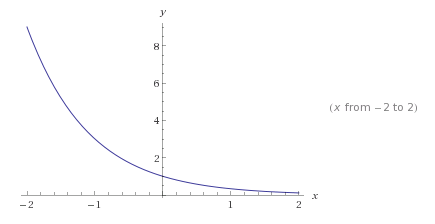
\includegraphics[scale=0.7]{figures/3_negative_x.png}

\end{document}

